\documentclass[10pt]{article}
\usepackage[document]{ragged2e}
\usepackage{multicol}
\usepackage[margin=1in]{geometry}
\usepackage{titlesec}
\usepackage{fancyhdr}
\usepackage{graphicx}
\graphicspath{ {./images/} }
\usepackage[justification=centering]{caption}
\captionsetup[subfigure]{justification=centering}
\captionsetup[figure]{justification=centering}
\usepackage{subcaption}
\usepackage{float}
\usepackage{enumitem}


\pagestyle{fancy}
\fancyhf{}
\fancyfoot[R]{Page. \thepage}
\fancypagestyle{plain}{
    \renewcommand{\headrulewidth}{0pt}
    \fancyhf{}
    \fancyfoot[R]{Page. \thepage}
}

\setlength{\parindent}{0em}
\setlength{\parskip}{1em}
\titlespacing*{\section}{0pt}{0.2em}{0.5em}
\titlespacing*{\subsection}{0pt}{0.2em}{0.2em}
\titlespacing*{\subsubsection}{0pt}{0.2em}{0.2em}


\title{Final Report}
\author{The Freedom Deer: Tianchang Li, Hualiang Qin, Qingwei Lan}

\begin{document}
\maketitle



\section*{Theme}

Our main goal is to investigate the conditions under which police officers tend to use force on civilians. We revolve our research on the differentiated treatments civilians receive from the police officers by studying the characteristics of the cases involved in the complaint and tactical response report. 

We want to know how the race of victims and race of officers play a role in the use of force cases respectively. Also, whether there is cross-race interaction influencing the likelihood of use of force. Under each race, we will look into the environmental factors that could work together to influence the decisions of the force usage. We hypothesize that environmental factors like visibility and place have an effect on the probability of the occurrence of force usage. Ultimately, we want to answer two questions:

\begin{enumerate}[noitemsep]
\item What makes someone riskier towards experiencing police use of force?
\item What are the typical scenarios in which police officers tend to use force?
\end{enumerate}



\section*{Checkpoint 1: Relational Analytics}

We started our research by exploring the racial distribution of officers and subjects in use of force cases. We looked at the racial composition of the subjects in use of force cases and compared it to the racial distribution of the entire population in Chicago. Results showed that Black subjects are the dominant race and contributed to more than 75\% of all use of force case subjects while making up only 30\% of the total population.

We hypothesized that an officer who is of a different race than the subject is more prone to use force (we call this “cross-race use of force”). Results showed that 73\% of total use of force cases involve cross-race use of force. This raises an interesting question regarding the dynamics of officers and subjects and led us to dig deeper into cross-race use of force cases later in our research.

One other interesting finding regarding use of force cases is that only 1.5\% of all cases involved firearm usage, which is quite low considering how widespread firearm usage is covered in the press.

We further looked at background factors that we hypothesized may have an impact on an officer’s decision to use force, namely: weather conditions, lighting conditions, indoors or outdoors, and location) and discovered that most of the cases happened outdoors under good lighting and weather conditions. Further analysis showed that these conditions do not differ significantly for subjects of different races.



\section*{Checkpoint 2: Data Visualization}

Our group then dug a little further in the demographics of the police officers and subjects involved in use-of-force cases, including race and age, and environmental factors, including the lighting, weather, and physical location, that help describe the scenarios where use-of-force occurred. 

To obtain an objective view of the race distribution of use-of-force subjects, we set up a baseline with the race distribution of the whole population. Compared to this baseline, we have found that all race groups make up lower percentages of subjects than the percentages of population except for the black group. Black group has a percentage of subjects that doubled its percentage in the population (Figure \ref{img1}). This anomaly indicates potential discrimination of police officers towards Black population. Besides, overall, Black, Hispanic, and White groups account for the majority of the cases.

\begin{figure}[H]
\captionsetup{font=small}
    \begin{subfigure}{0.5\textwidth}
        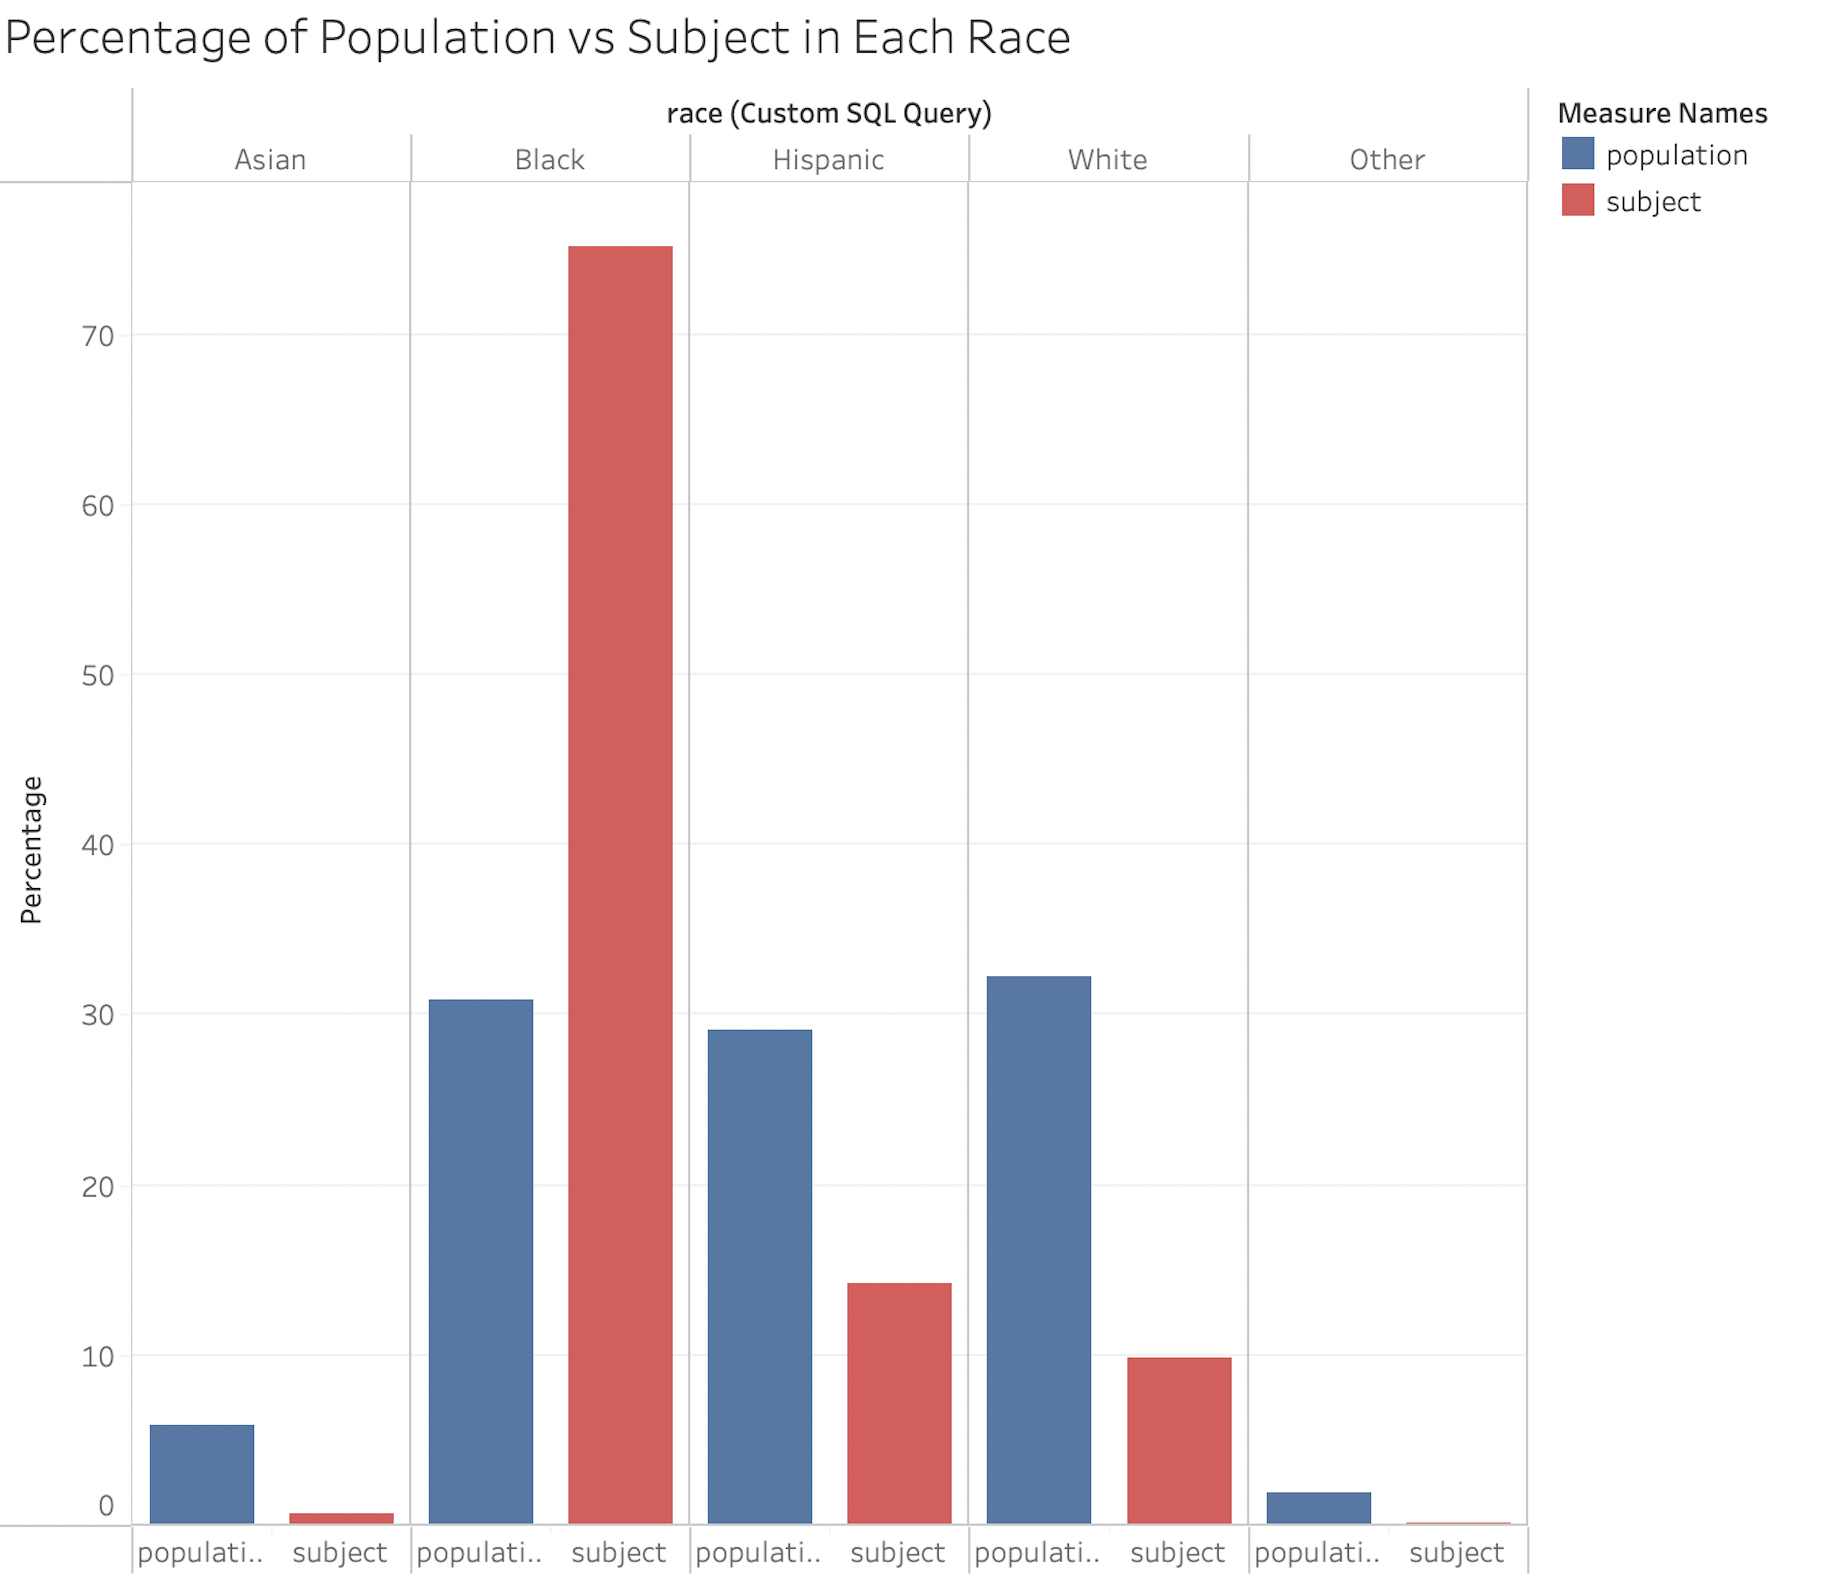
\includegraphics[width=\textwidth]{img1}
        \caption{Barcharts of (1) the percentage of the population of each race compared to the total population and (2) the percentage of use of force cases on subjects of each race compared to total use of force cases}
        \label{img1}
    \end{subfigure}%
    \begin{subfigure}{0.5\textwidth}
        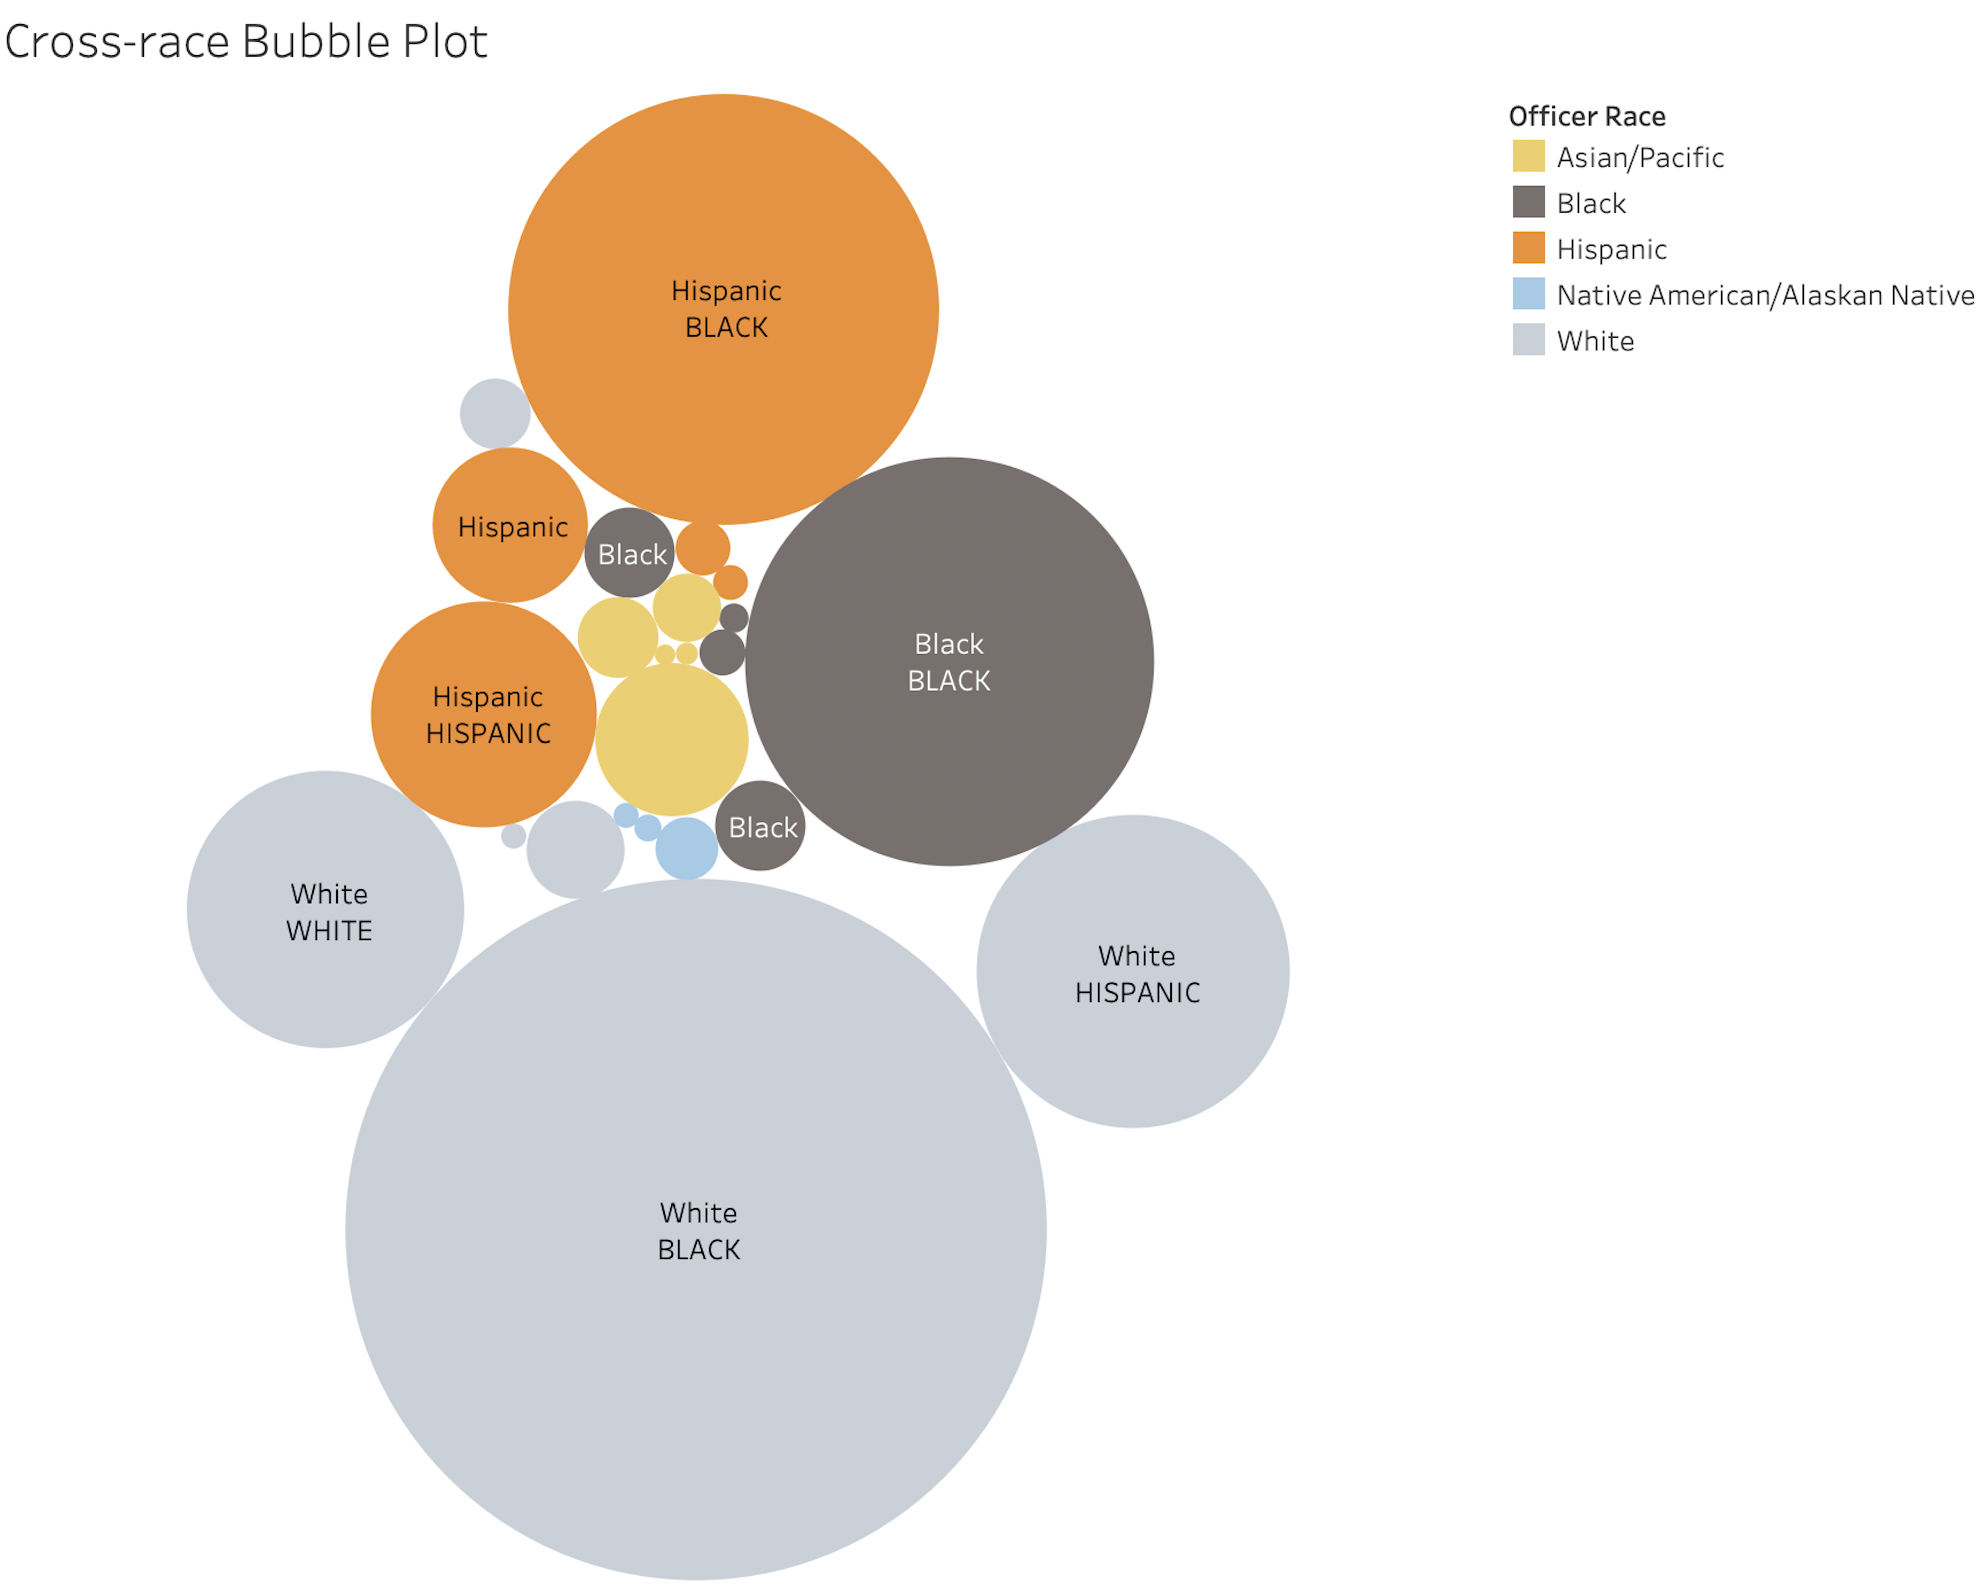
\includegraphics[width=\textwidth]{img3}
        \caption{Bubble plot depicting cross-race use of force cases}
        \label{img3}
    \end{subfigure}
\caption{Racial composition graphs}
\end{figure}

With this finding in race groups, we then branched off to explore other factors with their differentiations among races. By generating box plots in Figure \ref{img2}, we found that Black, Hispanic, and White groups have age spans across the board and on average are older than Asian, Native American, and other groups. We think there are stories hidden behind this straightforward finding. The lower average age in Asian and other race groups might result from the recent immigration waves, where lots of young adults came to the US. On the other hand, most Black, Hispanic, and White groups have lived in the country for a longer time. When each race group was further divided into gender groups, we did not see a prominent difference between male and female among races.

\begin{figure}[H]
\centering
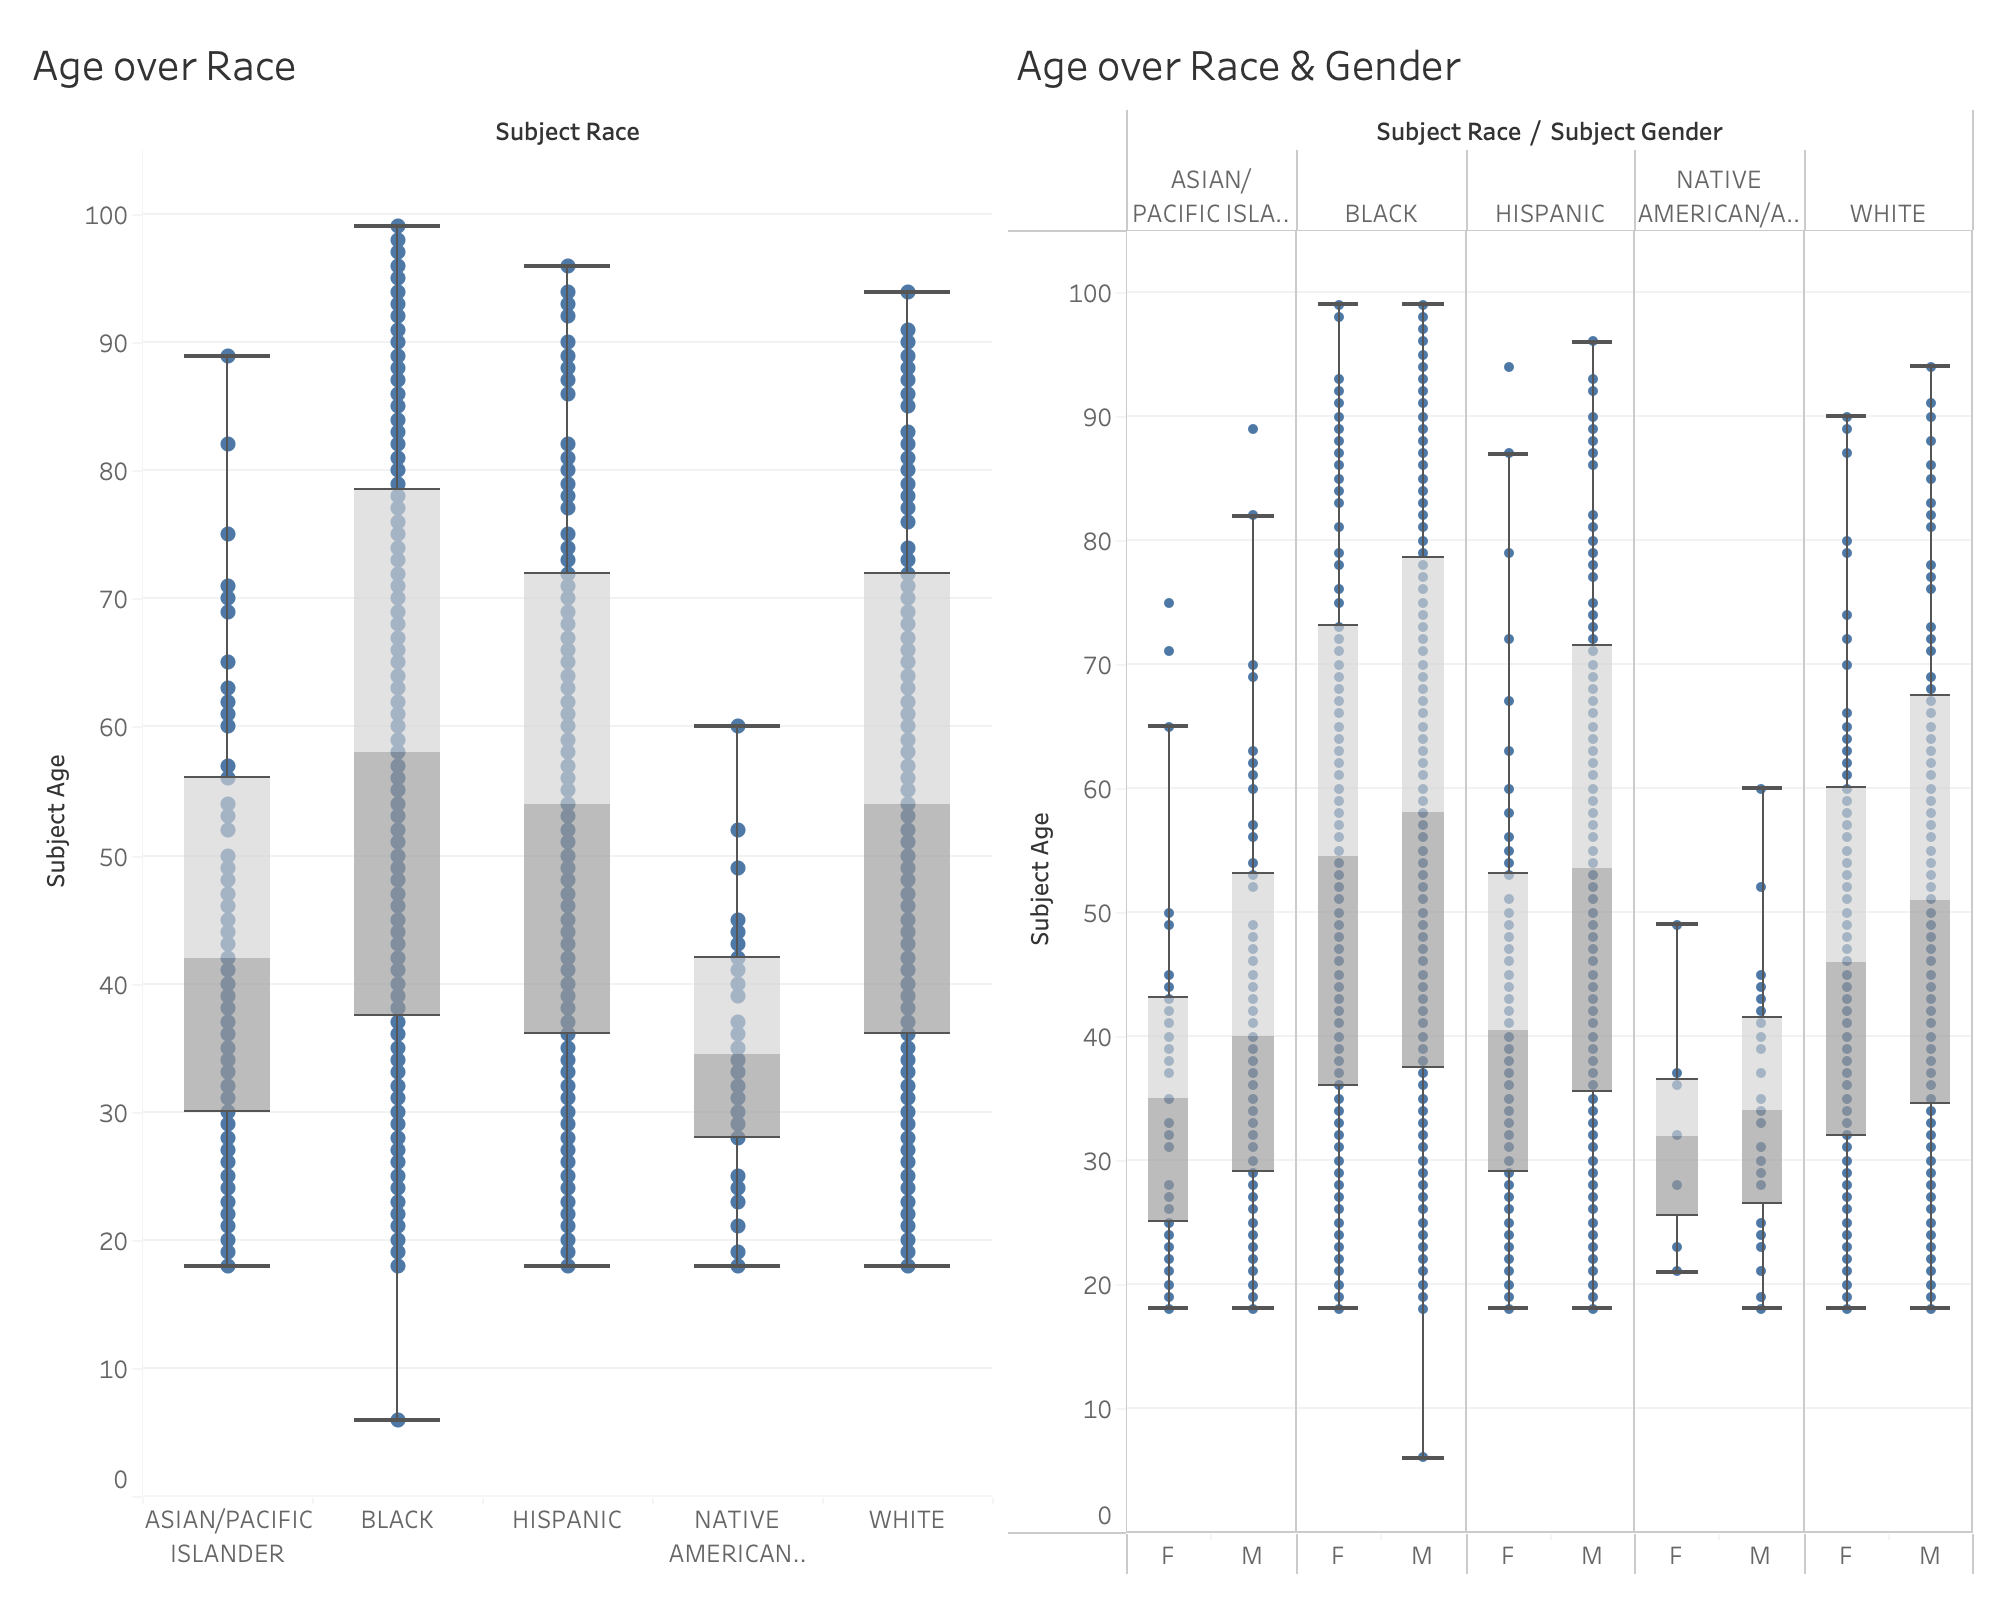
\includegraphics[width=0.75\textwidth]{img2}
\caption{Box and whisker plot of subject age over race and gender}
\label{img2}
\end{figure}

We also investigated the role that the race interaction between officers and subjects played in use-of-force cases. By generating the bubble plot in Figure \ref{img3}, we saw a prominently larger group of cases with White officers and Black subjects. The second largest group being Hispanic officers and Black subjects. In fact, three out of the top five race combinations are cross-race. This indicates a potential bias police officers hold to out-of-group individuals.

Finally, we explored the environmental factors that are the most common in use-of-force cases as well as their difference among race groups. We saw that cases usually occurred under daylight or good artificial light, clear weather, and outdoors on the street (Figure 3). These all indicate rather good visibility on the spot. It could be interpreted as that police officers usually could and might have identified suspicious activities of subjects before exercising force, which is relieving to see. However, we did not see a clear difference among race groups in terms of certain environments.

\begin{figure}[H]
\captionsetup{font=small}
    \begin{subfigure}{0.5\textwidth}
        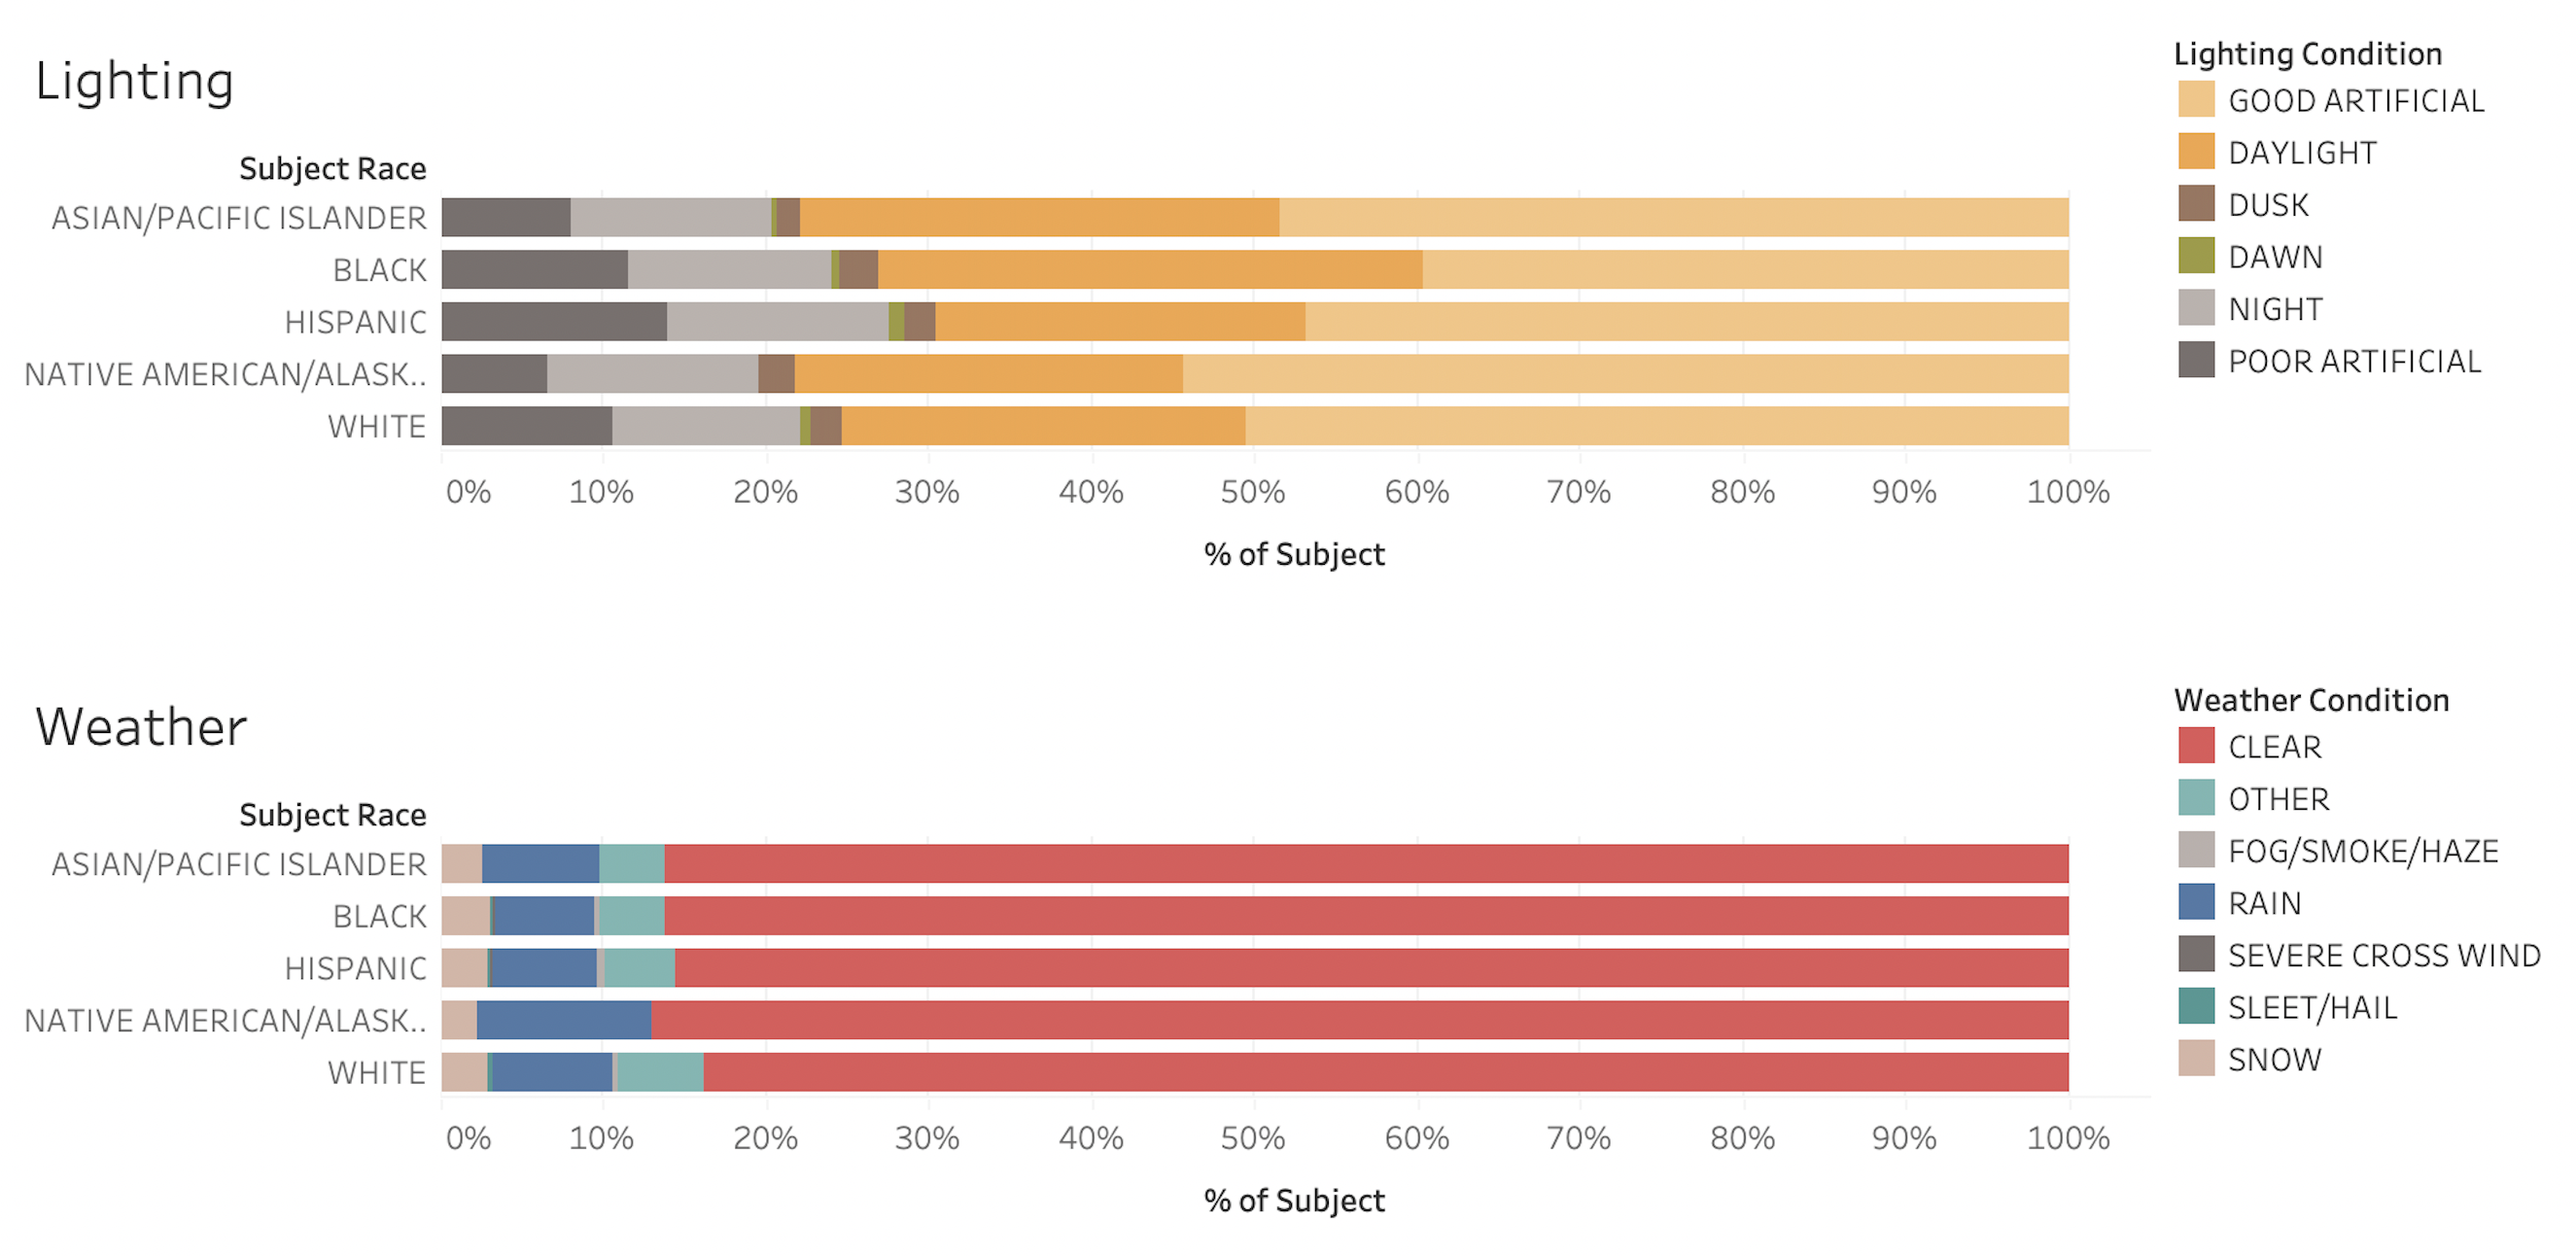
\includegraphics[width=\textwidth]{img4}
        \label{img4}
    \end{subfigure}%
    \begin{subfigure}{0.5\textwidth}
        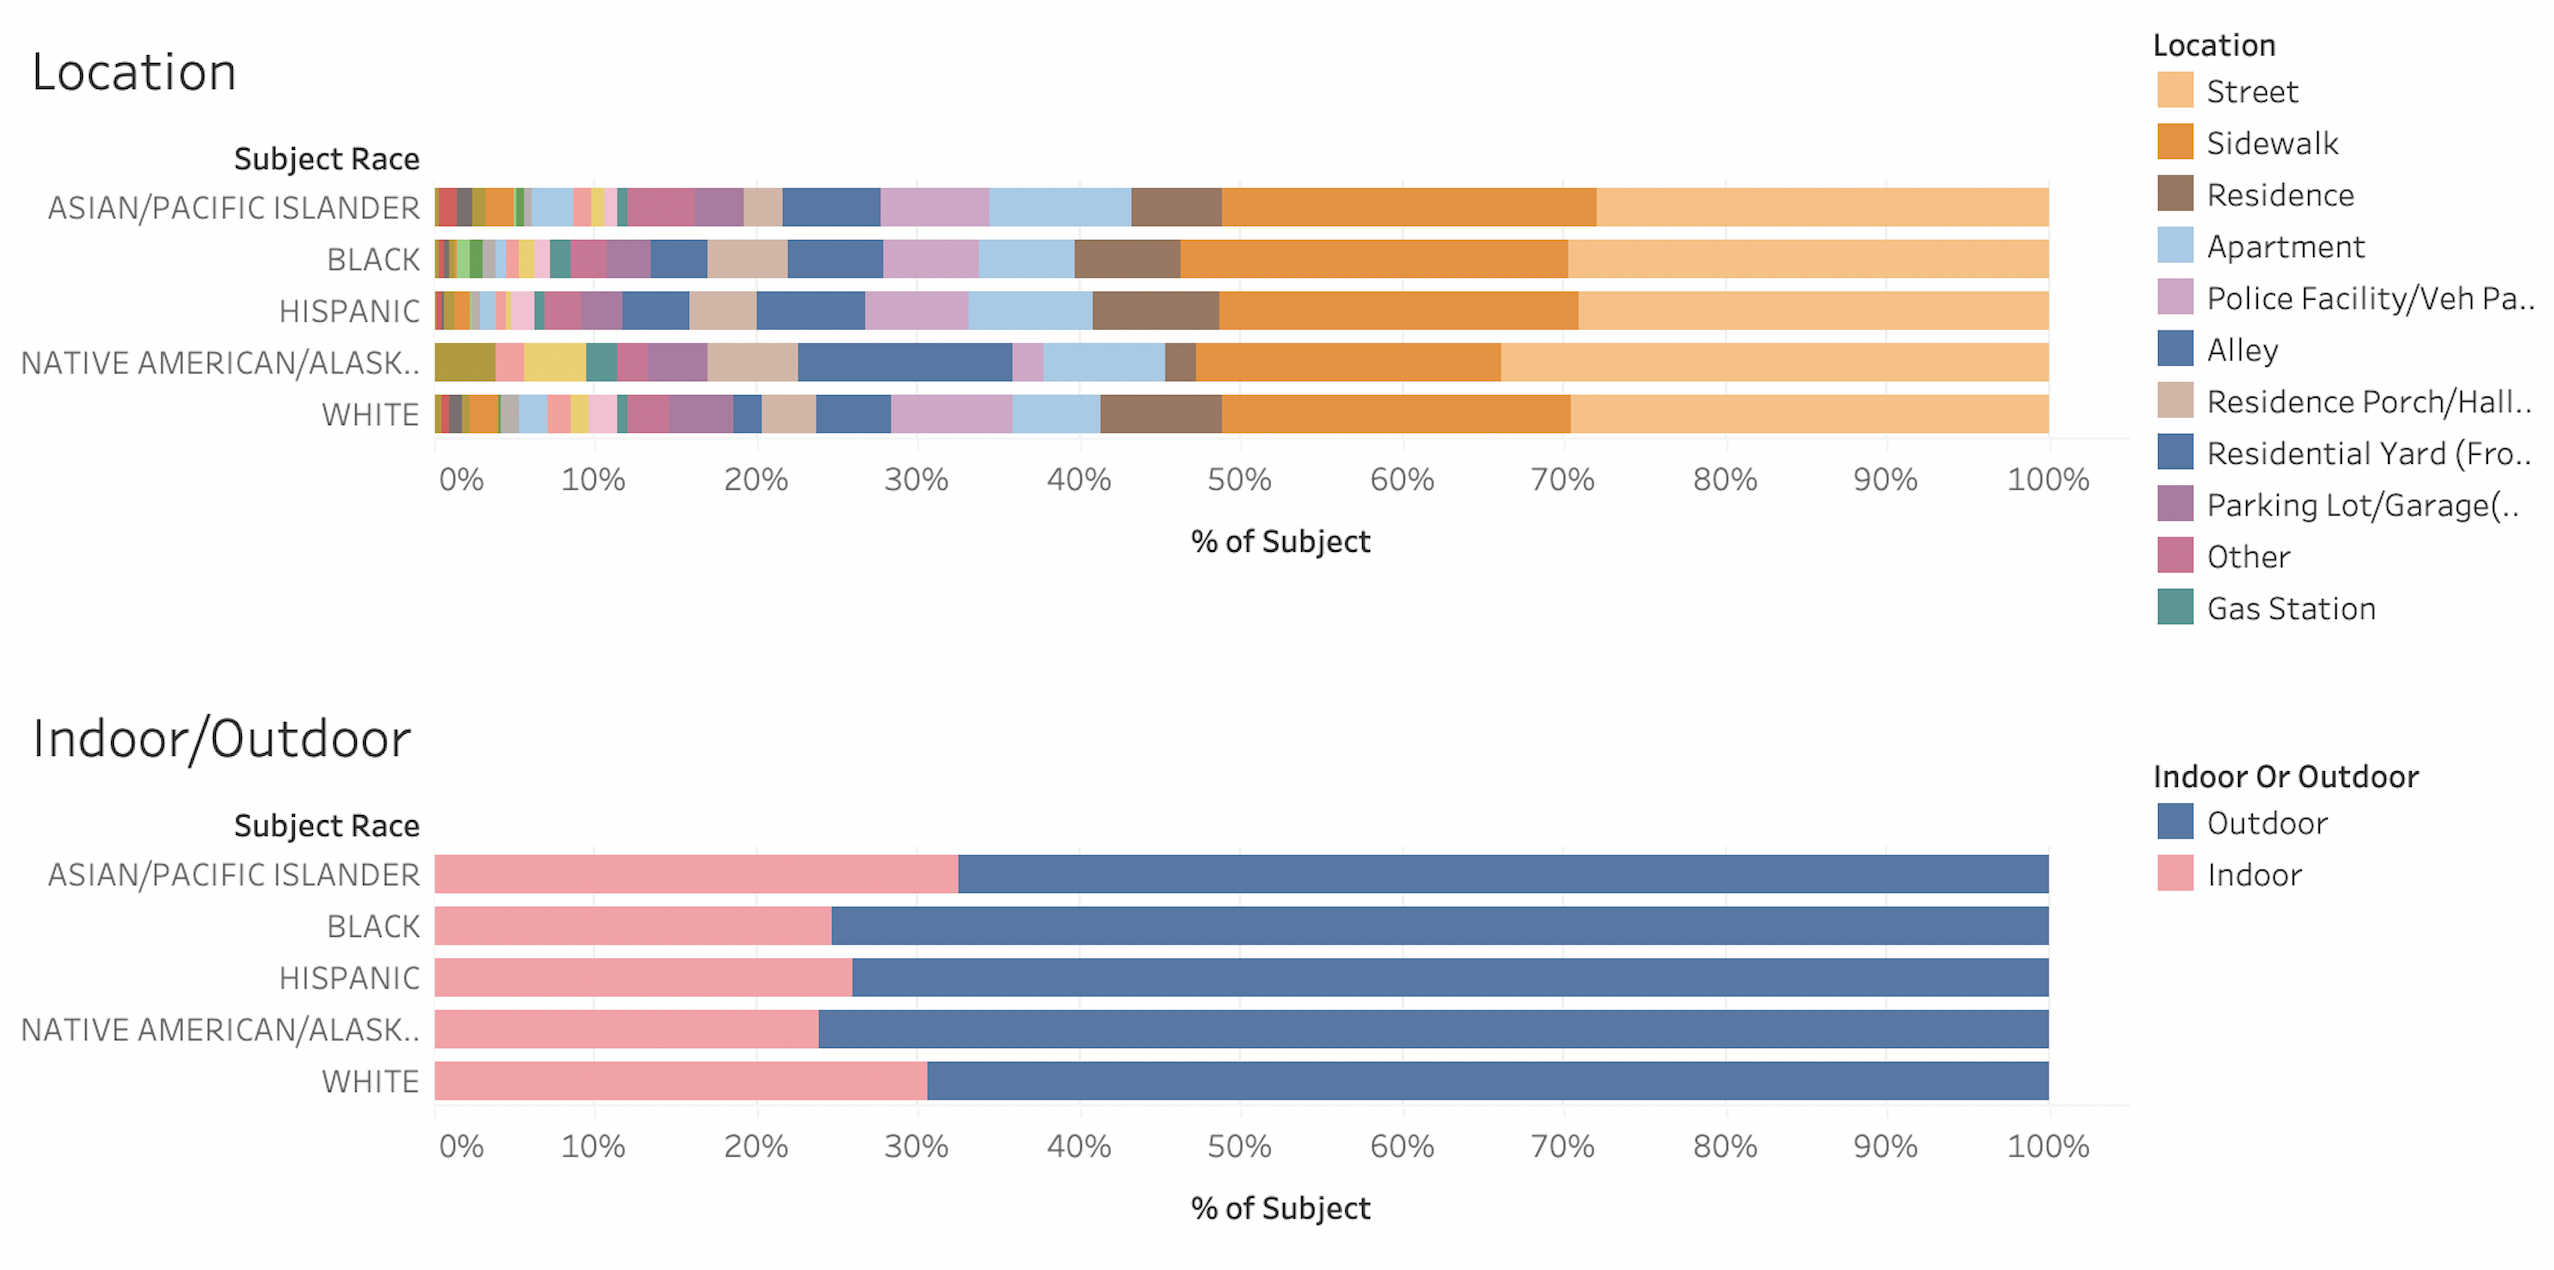
\includegraphics[width=\textwidth]{img5}
        \label{img5}
    \end{subfigure}
\label{barcharts}
\caption{Barcharts of the frequency of police use of force cases in different environmental conditions (lighting, weather, location, indoors/outdoors) over each race}
\end{figure}



\section*{Checkpoint 3: Interactive Visualization}

For interactive visualization, we first looked into an interactive bubble chart to see if cross race combinations change every three years from 2004 to 2016\footnote{https://observablehq.com/@c69ef2da2b4d284b/bubble-plot-of-cross-race}. As time went by, the fact that Black subjects made up about 70\% of the total subjects and the White officers made up about 60\% of total officers doesn’t change over the years, nor do the top cross race combinations.

We also use an interactive top k bar chart to examine if firearm usage would make a difference of the effect of various environmental factors\footnote{https://observablehq.com/@c69ef2da2b4d284b/bar-chart-horizontal-environmental-factor-on-use-of-force}. The conclusion is the top one condition of each environmental factor made up more occurrences when firearms were involved. If we consider the usage of firearms as an escalation of the general use of force case, it is reasonable that firearm usage reinforced and relied more on the environment where force usage is more likely to happen.

In terms of the demographic information of the subject and officer, we inspected it with a sunburst graph\footnote{https://observablehq.com/@ltcrazy/sequence-sunburst-portraiting-the-demographics-of-the-2-pa}. We found out that Black and Hispanic males between 18-40 year-old are the most risky to police’s use of force. Moreover, White and Hispanic males older than 40 year-old are prone to exercise violence. We suggest these groups be aware of such facts and risks.

After all, we have drawn a conclusion on the environmental factors at this checkpoint. Furthermore, the fact that the effects of environmental factors have no significant difference between races help us to make our decision to focus on exploring the role of race in the use of force cases and examine it with different tools and from different perspectives in the following checkpoints.



\section*{Checkpoint 4: Graph Analytics}

In this checkpoint, we ran graph analytics to determine whether there were a group of officers that accounted for the majority of TRR cases and whether these officers influenced other officers. We plot a network graph of co-offending officers with each node representing an officer and each edge connecting a co-offending pair of officers. In addition, we also plot the baseline graph where each node also represents an officer but each edge connects two officers if they appear in the same shift together. By comparing these two graphs (Figure 4), we can see that the co-offending graph is tightly connected whereas the baseline graph is sparse. This shows that the top co-offending officers do not work in the same shifts. The graph comparisons do not differ significantly between cross-race vs. all TRR cases (Figures 4 \& 5).

\begin{figure}[H]
\centering
\captionsetup{font=small}
    \begin{subfigure}{0.5\textwidth}
        \frame{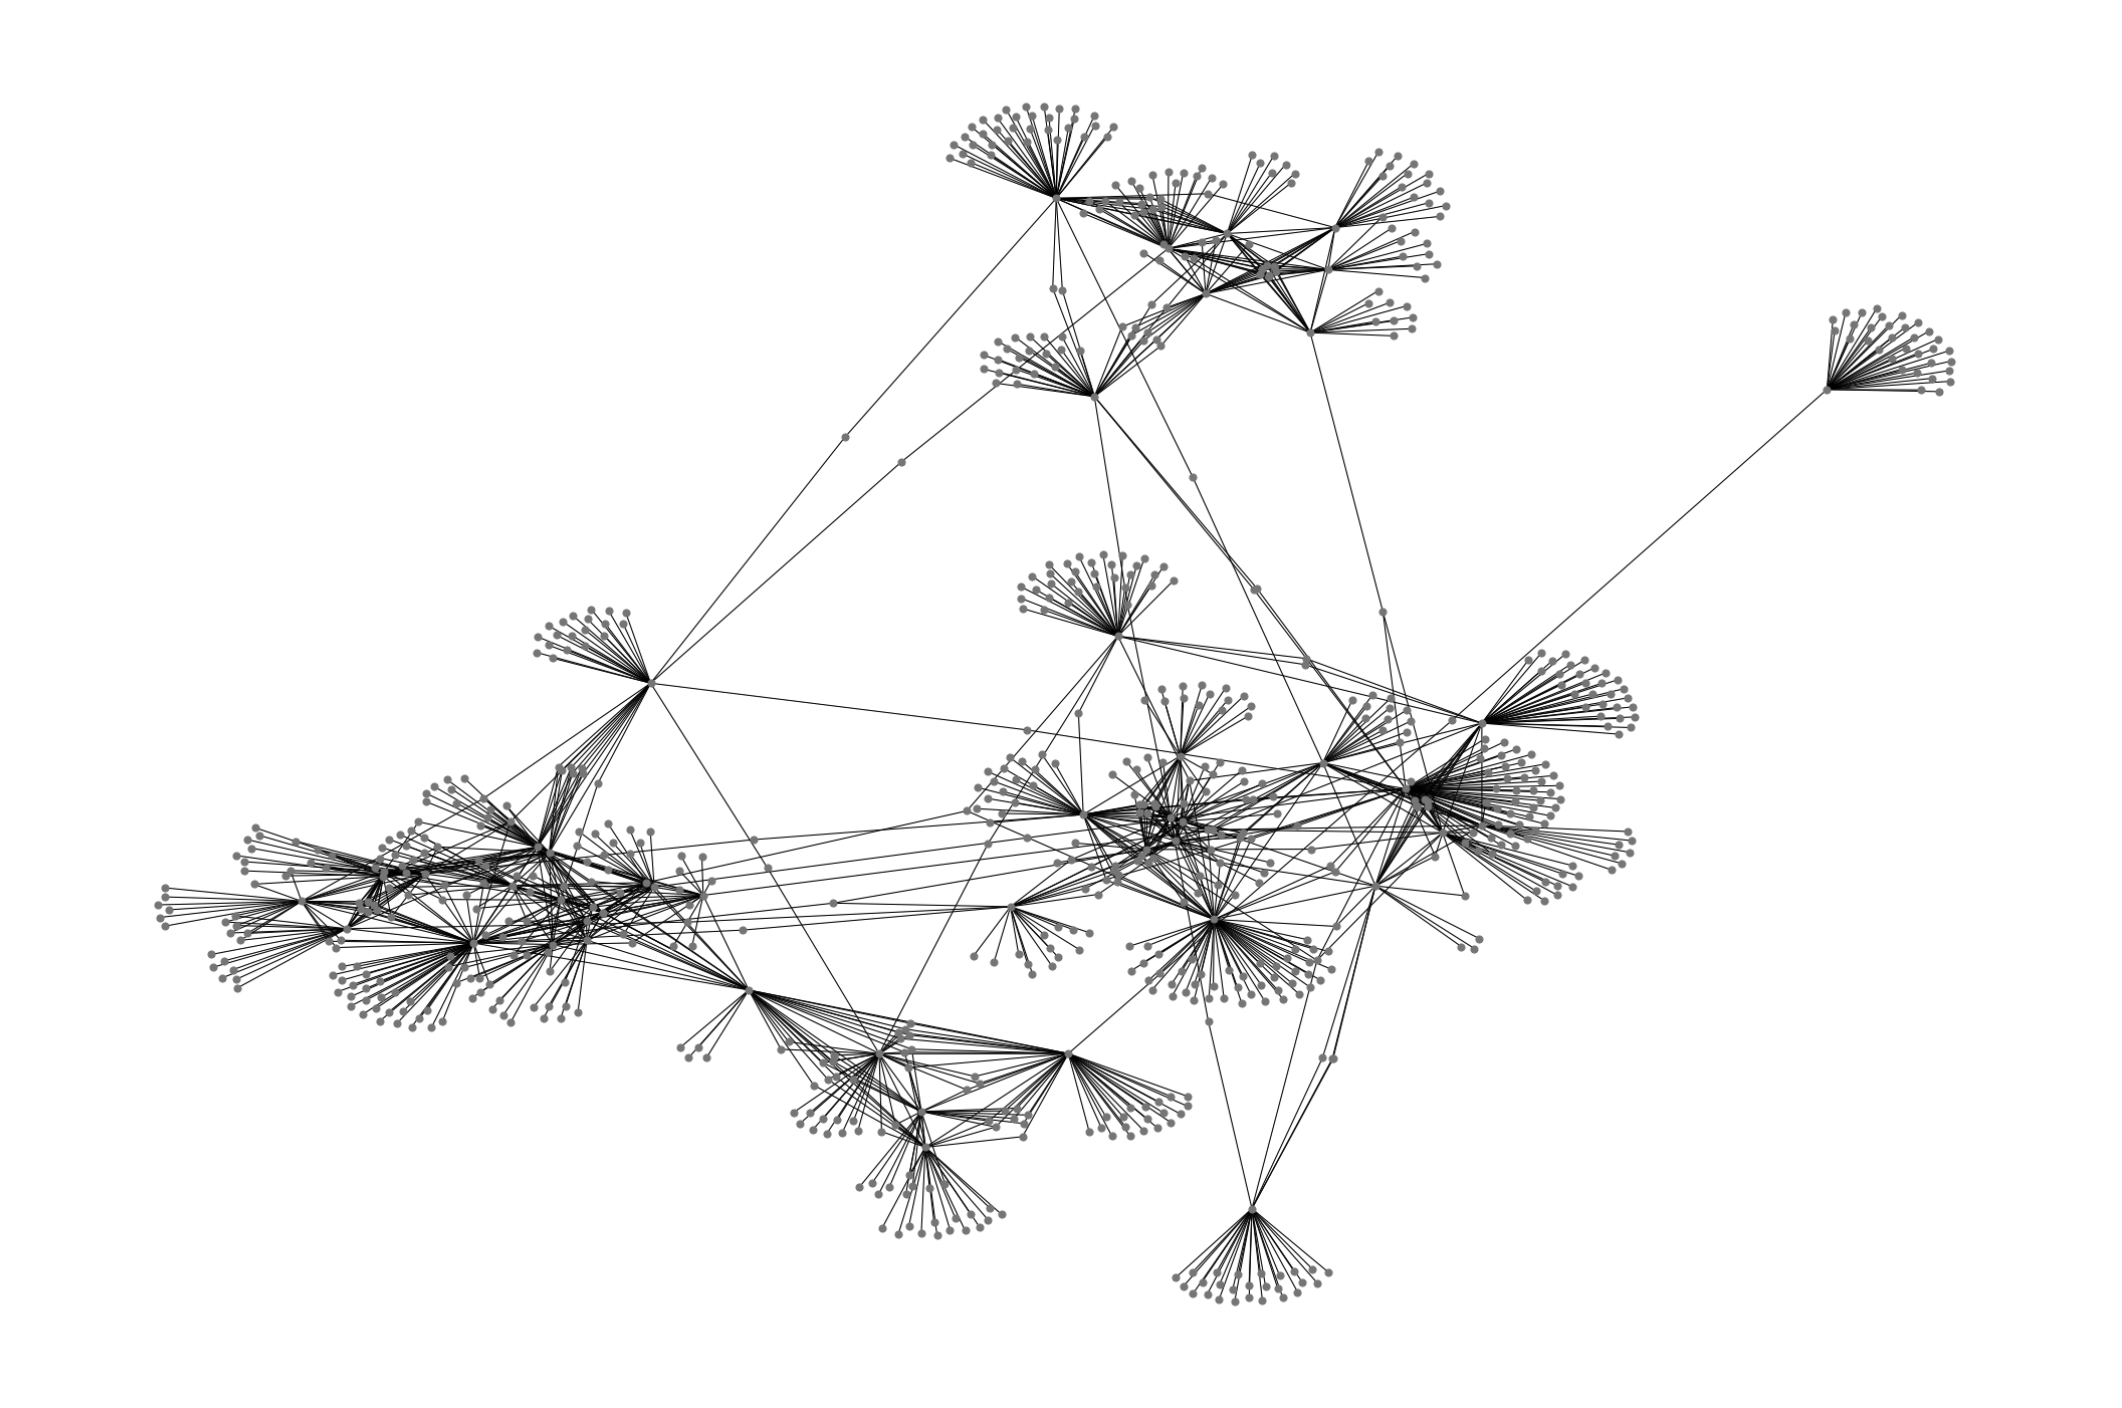
\includegraphics[width=\textwidth]{trr}}
        \caption{TRR network graph}
        \label{trr}
    \end{subfigure}%
    \begin{subfigure}{0.5\textwidth}
        \frame{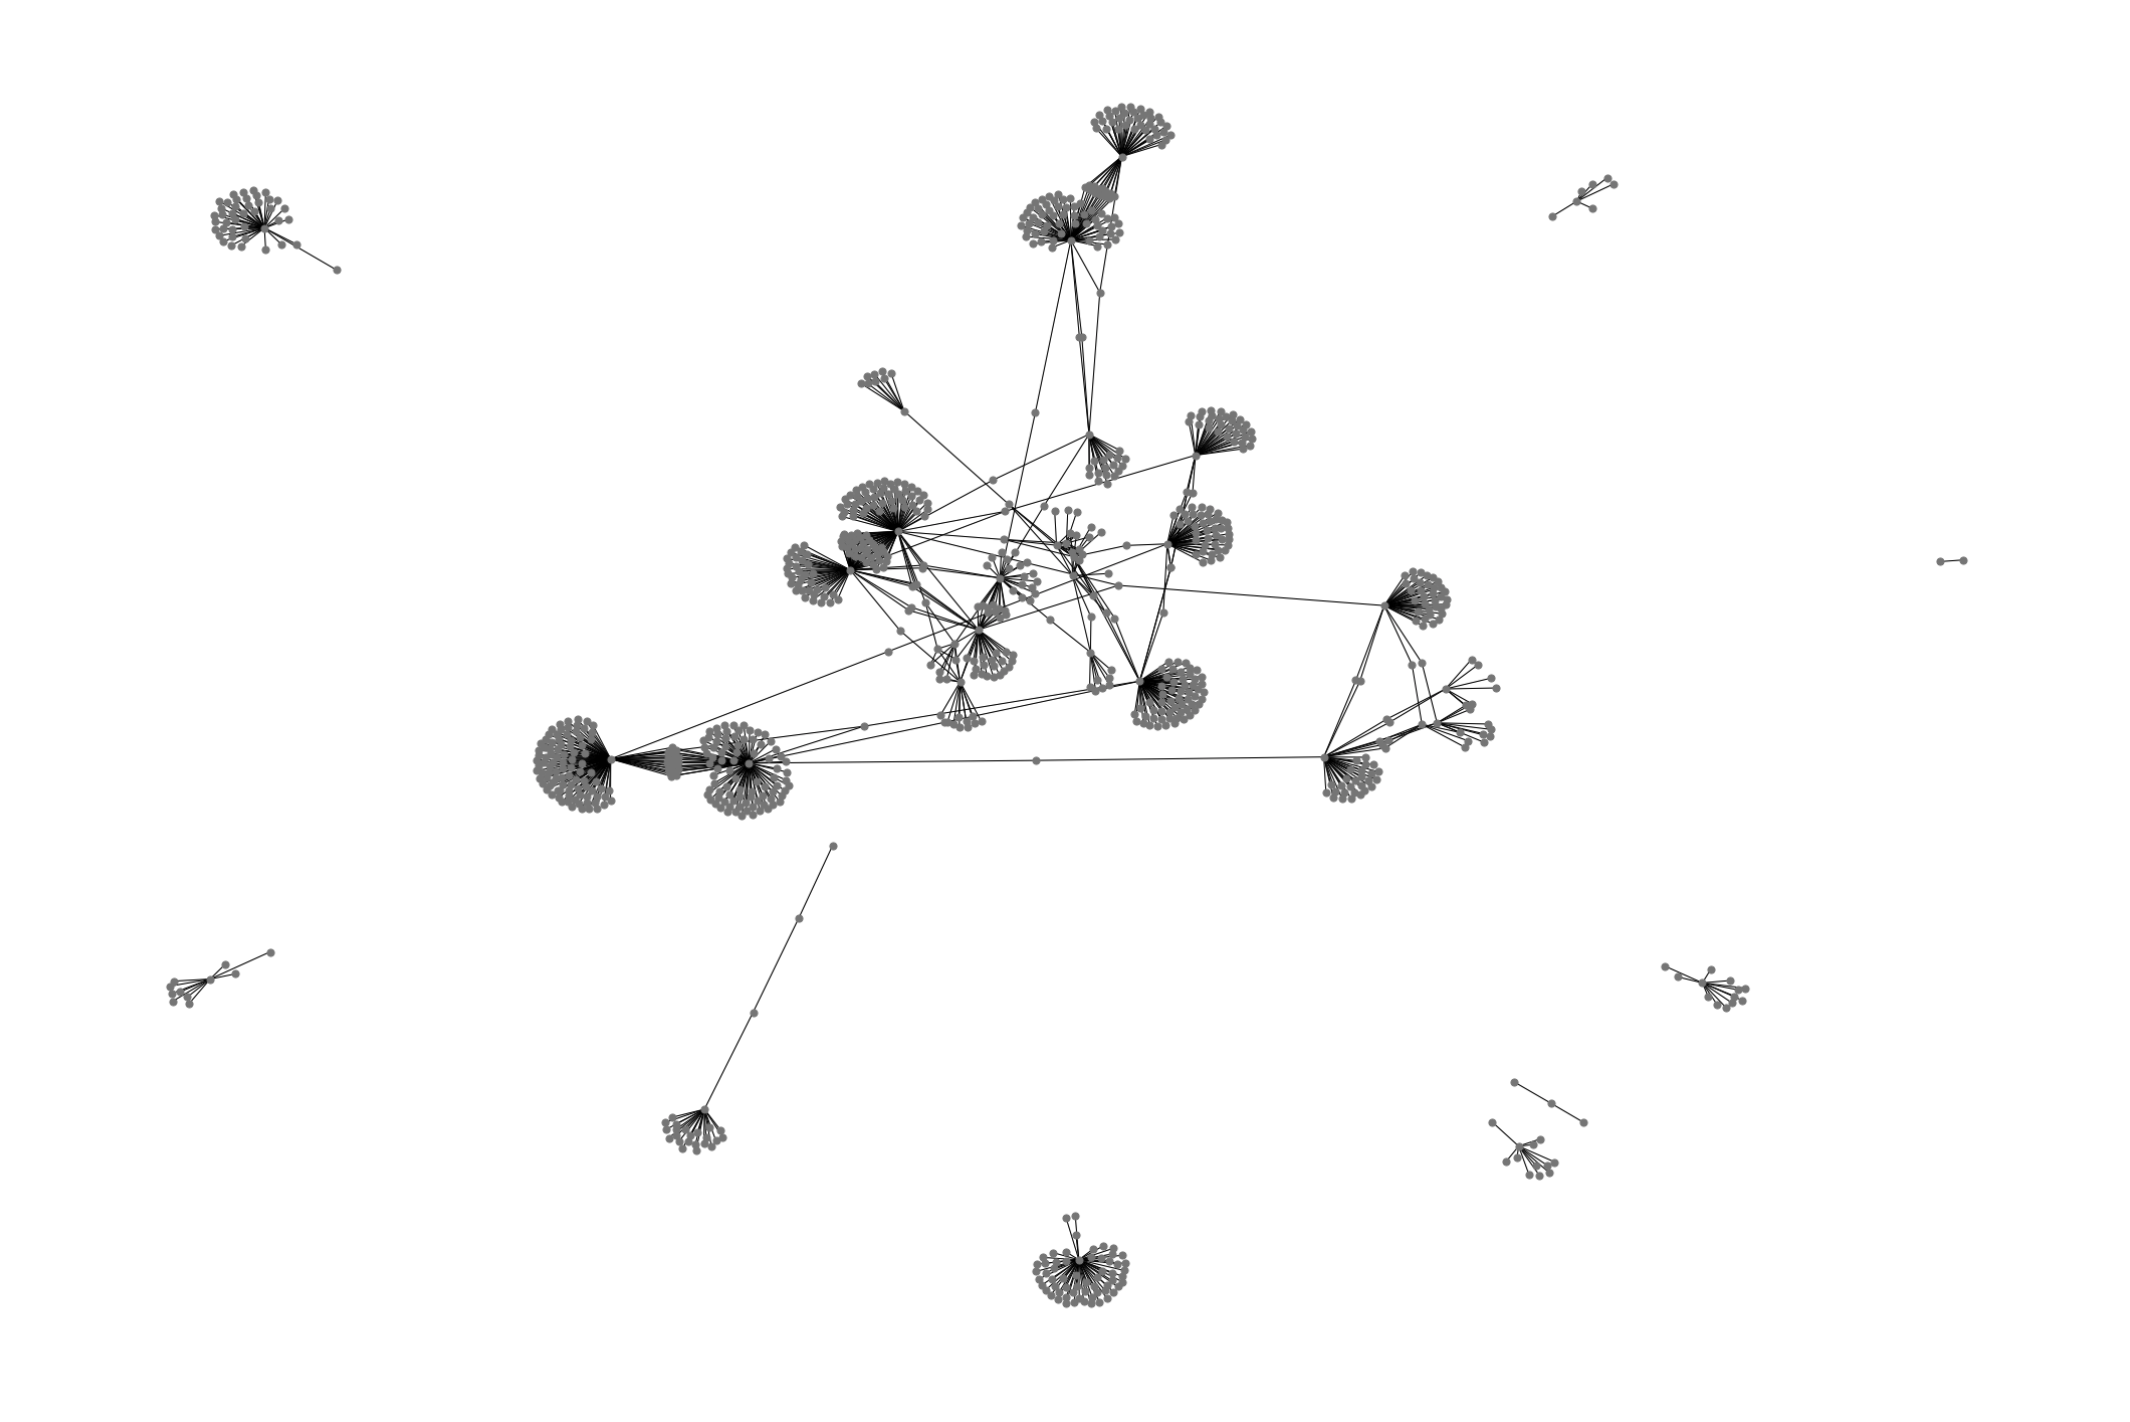
\includegraphics[width=\textwidth]{baseline}}
        \caption{Baseline network graph}
        \label{baseline}
    \end{subfigure}
\caption{TRR network graph and baseline network graph for all TRR cases.}
\end{figure}


\begin{figure}[H]
\centering
\captionsetup{font=small}
    \begin{subfigure}{0.5\textwidth}
        \frame{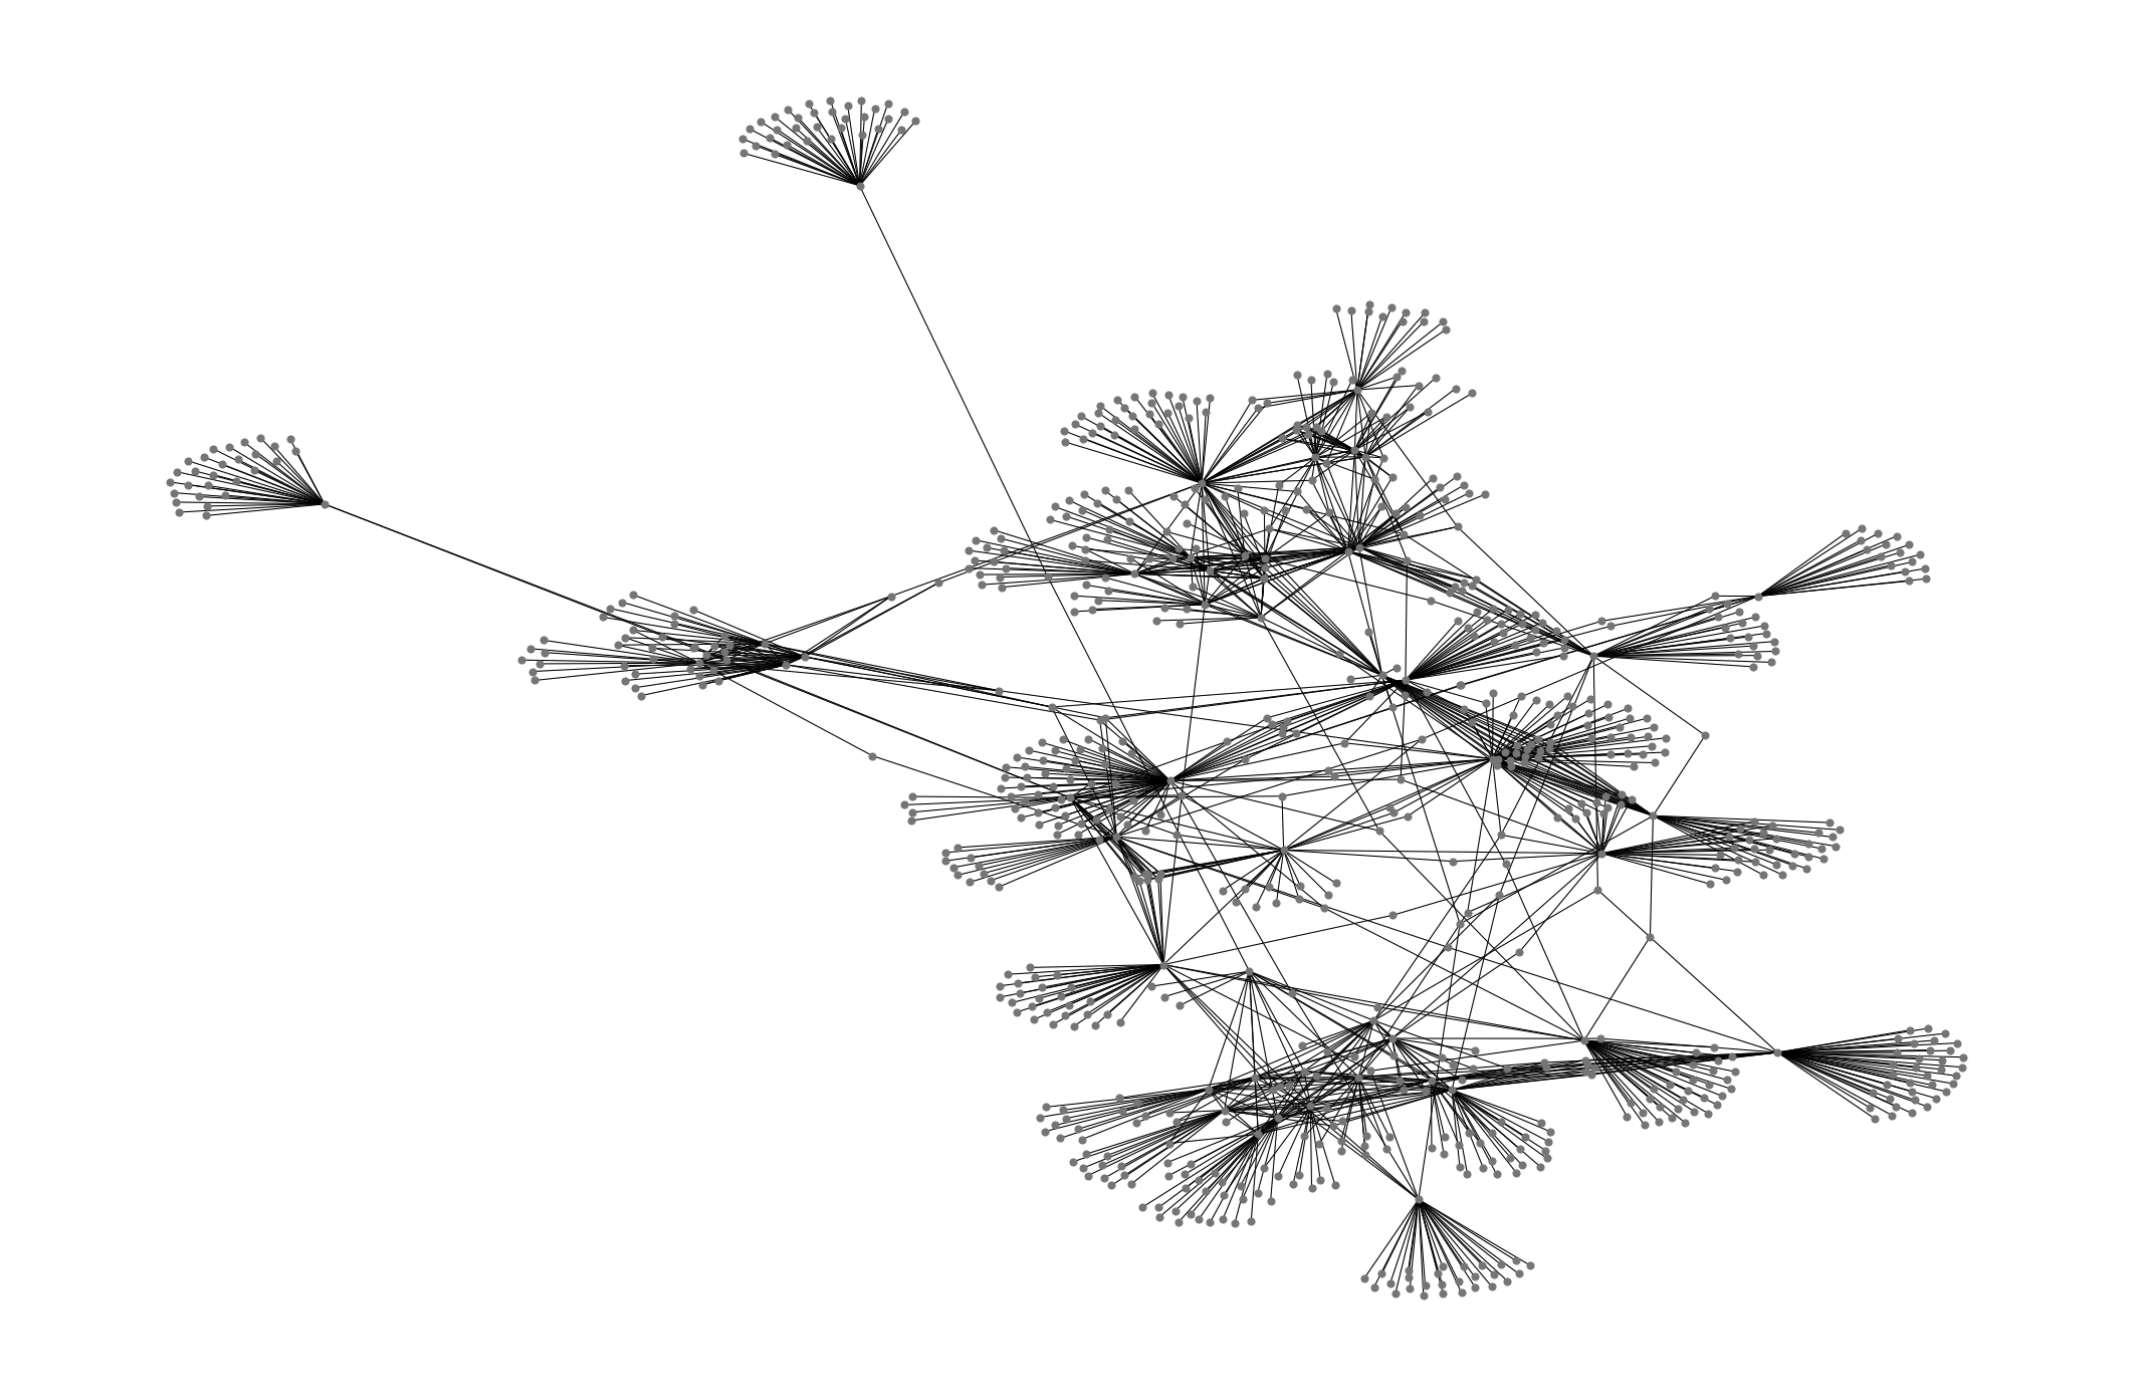
\includegraphics[width=\textwidth]{trr_cross_race}}
        \caption{TRR network graph}
        \label{trr_cross_race}
    \end{subfigure}%
    \begin{subfigure}{0.5\textwidth}
        \frame{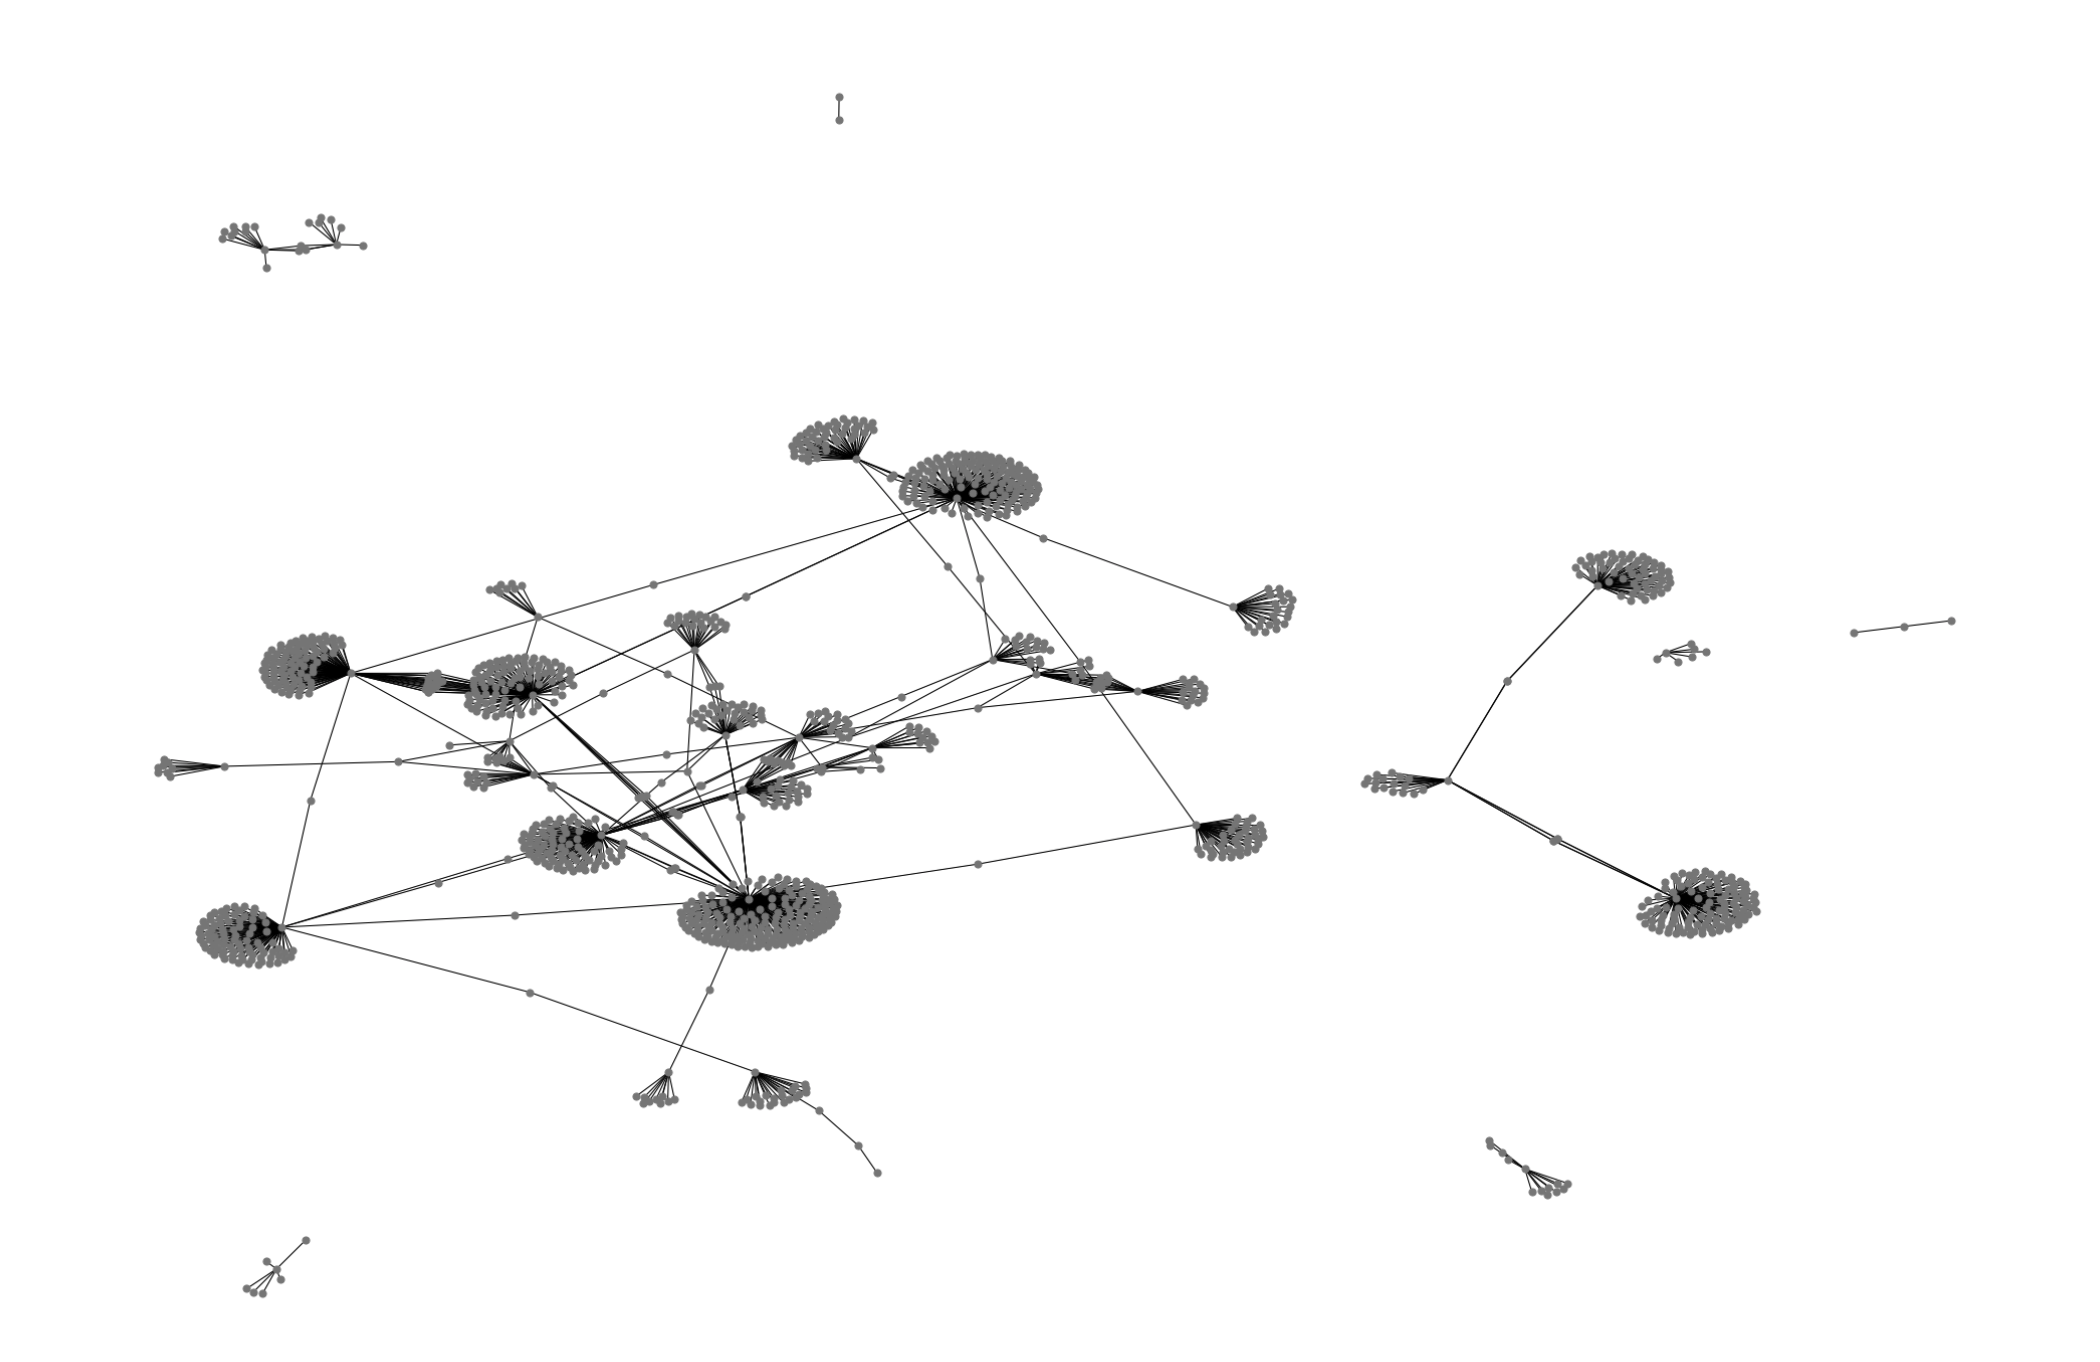
\includegraphics[width=\textwidth]{baseline_cross_race}}
        \caption{Baseline network graph}
        \label{baseline_cross_race}
    \end{subfigure}
\caption{TRR network graph and baseline network graph for TRR cases involving only \textbf{cross-race use of force}.}
\end{figure}

To dig deeper into the network effects, we ran the triangle count algorithm and page rank algorithm to determine the most “influential” officers. The results agree with our network graphs but don’t really provide much extra information. We also investigated the difference between on-shift and off-shift use-of-force cases for the most influential officers by performing individual-level analysis on them, given that off-shift use of force commonly comes out of bad intention. However, we did not see a prominent difference. This indicates that off-shift, so far, is not a big concern in need of strict regularization.



\section*{Checkpoint 5: Natural Language Processing}

In this checkpoint, we extended one of our previous exploratory findings which showed considerably more cross-race cases in use of force, meaning that the police officer and subject involved are from different race groups, than same-race cases. Here, we are interested in investigating the role race plays in police misconduct.

We hypothesized that how severe a police misconduct is depends on how necessary it is given the accusation scenario, the race of police officer and subject, and some other factors. By looking at the statistical significance of race variable(s), we assessed whether using force is escalated by certain race compositions, controlling for the accusation and other factors.

We investigated the role race plays in police use of force by assessing the situation with a sentimental analysis and running regression analyses, controlling for the sentimental scores. We discovered that being white is not necessarily a factor for police to use force but being black could be a factor that encourages police use of force. More importantly, police misconduct is evidently escalated if officers and subjects come from different race groups.



\section*{Conclusion}

Through the various aspects of analyses we performed on CPDB, we were able to portray the nature of police officers and subjects involved in use-of-force cases. We found that White and Hispanic male officers older than 40 year-old are prone to exercise violence. On the other hand, Black and Hispanic males between 18-40 year-old are the most risky to police’s use of force. Particularly, cross-race interaction played an important role in escalating the severity of police misconduct. In terms of environment, use of force usually occurred under good lighting and outdoors on the streets. Among police officers, the network is much tighter than their assigned shifts, which indicates abnormal bondings formed within the crews that exercise force.

We highly recommend the Chicago police department to form internal training that emphasizes the anomalies and potential biases accordingly. With our findings, we also hope to remind the individuals in the risky groups to be aware of such risks and take actions to protect themselves when needed. 



\section*{Future Direction}

In Checkpoint 3, when we are examining the demographic information of subjects and officers, we make our conclusion that White males and Hispanic males older than 40 year-old are prone to exercise violence. This conclusion would be more convincing and insightful if we take the CPD population into consideration as a baseline and enrich our conclusion by the comparison with the baseline.

This is related to a concerned issue that radiates to many aspects in the studies of CPDB, which is the extremely unbalanced race composition of officers and subjects in the dataset. Future researchers should enrich the dataset by integrating diverse records from other police departments, if they want to draw more generalizable conclusions on race impacts.

More importantly, for a bigger picture, we want to answer the question: what is the in-depth nature of the incident that leads to use of force? For which we can monitor the officers' groups to encourage restraining use of force. For the sunburst visualization itself, it would be more insightful if we can look into the action response data in CPDB and depict its timeline. Hopefully it could help us to answer the question.


\end{document}
